%=======================02-713 LaTeX template, following the 15-210 template==================
%
% You don't need to use LaTeX or this template, but you must turn your homework in as
% a typeset PDF somehow.
%
% How to use:
%    1. Update your information in section "A" below
%    2. Write your answers in section "B" below. Precede answers for all 
%       parts of a question with the command "\question{n}{desc}" where n is
%       the question number and "desc" is a short, one-line description of 
%       the problem. There is no need to restate the problem.
%    3. If a question has multiple parts, precede the answer to part x with the
%       command "\part{x}".
%    4. If a problem asks you to design an algorithm, use the commands
%       \algorithm, \correctness, \runtime to precede your discussion of the 
%       description of the algorithm, its correctness, and its running time, respectively.
%    5. You can include graphics by using the command \includegraphics{FILENAME}
%
\documentclass[11pt]{article}
\usepackage{amsmath,amssymb,amsthm}
\usepackage{graphicx}
\usepackage[margin=1in]{geometry}
\usepackage{fancyhdr}
\usepackage{listings}
\setlength{\parindent}{0pt}
\setlength{\parskip}{5pt plus 1pt}
\setlength{\headheight}{13.6pt}
\newcommand\question[2]{\vspace{.25in}\hrule\textbf{#1: #2}\vspace{.5em}\hrule\vspace{.10in}}
\renewcommand\part[1]{\vspace{.10in}\textbf{(#1)}}
\newcommand\algorithm{\vspace{.10in}\textbf{Algorithm: }}
\newcommand\correctness{\vspace{.10in}\textbf{Output: }}
\newcommand\runtime{\vspace{.10in}\textbf{Running time: }}
\pagestyle{fancyplain}
\lhead{\textbf{\NAME\ (\ANDREWID)}}
\chead{\textbf{Project\HWNUM}}
\rhead{\today}
\begin{document}\raggedright
%Section A==============Change the values below to match your information==================
\newcommand\NAME{Yao Xiao}  % your name
\newcommand\ANDREWID{2019180015}     % your andrew id
\newcommand\HWNUM{1}              % the homework number
%Section B==============Put your answers to the questions below here=======================

% no need to restate the problem --- the graders know which problem is which,
% but replacing "The First Problem" with a short phrase will help you remember
% which problem this is when you read over your homeworks to study.

\question{1}{Programming 1} 

\part{a} \algorithm The implement of Server
\begin{lstlisting}
import select
import socket
import struct
from socketserver import StreamRequestHandler, ThreadingTCPServer

SOCKS_VERSION = 5

class Socks5Proxy(StreamRequestHandler):
    def handle(self):
        print('Accepting connection from {}'.format(self.client_address))

        # read 2 bytes data from client
        header = self.connection.recv(2)
        version, nmethods = struct.unpack("!BB", header)
        
        # set socks5, nmethods
        assert version == SOCKS_VERSION
        assert nmethods > 0

        # 1.Get authentication method
        methods = self.get_methods(nmethods)
        
        # 2.Select method 0x00(NO AUTHENTICATION REQUIRED)
        if 0 not in set(methods):
            self.server.close_request(self.request)
            return
        self.connection.sendall(struct.pack("!BB", SOCKS_VERSION, 0))

        # 3.Requests
        version, cmd, _, address_type = struct.unpack("!BBBB", self.connection.recv(4))
        assert version == SOCKS_VERSION
        # DST.ADDR 
        # IPv4
        if address_type == 1:  
            address = socket.inet_ntoa(self.connection.recv(4))
        # Domain name       
        elif address_type == 3:  
            domain_length = self.connection.recv(1)[0]
            address = self.connection.recv(domain_length)
        # IPV6
        elif address_type == 4:  
            addr_ip = self.connection.recv(16)
            address = socket.inet_ntop(socket.AF_INET6, addr_ip)
        else:
            self.server.close_request(self.request)
            return
        port = struct.unpack('!H', self.connection.recv(2))[0]

        # Response to only connect 0x01
        try:
            if cmd == 1: 
                remote = socket.socket(socket.AF_INET, socket.SOCK_STREAM)
                remote.connect((address, port))
                bind_address = remote.getsockname()
                print('Connected to {} {}'.format(address, port))
            else:
                self.server.close_request(self.request)
            addr = struct.unpack("!I", socket.inet_aton(bind_address[0]))[0]
            port = bind_address[1]

          
		    # VER, CMD, RSV, ATYP, ADDR, PORT
            reply = struct.pack("!BBBBIH", SOCKS_VERSION, 0, 0, 1, addr, port)
        except Exception as err:
            logging.error(err)

            reply = self.failed_reply(address_type, 5)
        self.connection.sendall(reply)

        # connect success, change data
        if reply[1] == 0 and cmd == 1:
            self.exchange_loop(self.connection, remote)
        self.server.close_request(self.request)

    
    def get_methods(self, n):
        methods = []
        for i in range(n):
            methods.append(ord(self.connection.recv(1)))
        return methods

    def failed_reply(self, address_type, error_number):
        return struct.pack("!BBBBIH", SOCKS_VERSION, error_number, 0, address_type, 0, 0)

    def exchange_loop(self, client, remote):
        while True:
            r, w, e = select.select([client, remote], [], [])
            if client in r:
                data = client.recv(4096)
                if remote.send(data) <= 0:
                    break
            if remote in r:
                data = remote.recv(4096)
                if client.send(data) <= 0:
                    break


if __name__ == '__main__':
    # use ThreadingTCPServer to strat proxy 
    with ThreadingTCPServer(('127.0.0.1', 8848), Socks5Proxy) as server:
        server.serve_forever()
\end{lstlisting}

\part{b} \algorithm The implement of Client
\begin{lstlisting}
import socket
import socks 
import requests

socks.set_default_proxy(socks.SOCKS5, "127.0.0.1", 8848, username=None, password=None)
socket.socket = socks.socksocket
print(requests.get('http://www.baidu.com').text)
\end{lstlisting}

\part{c} \correctness\\
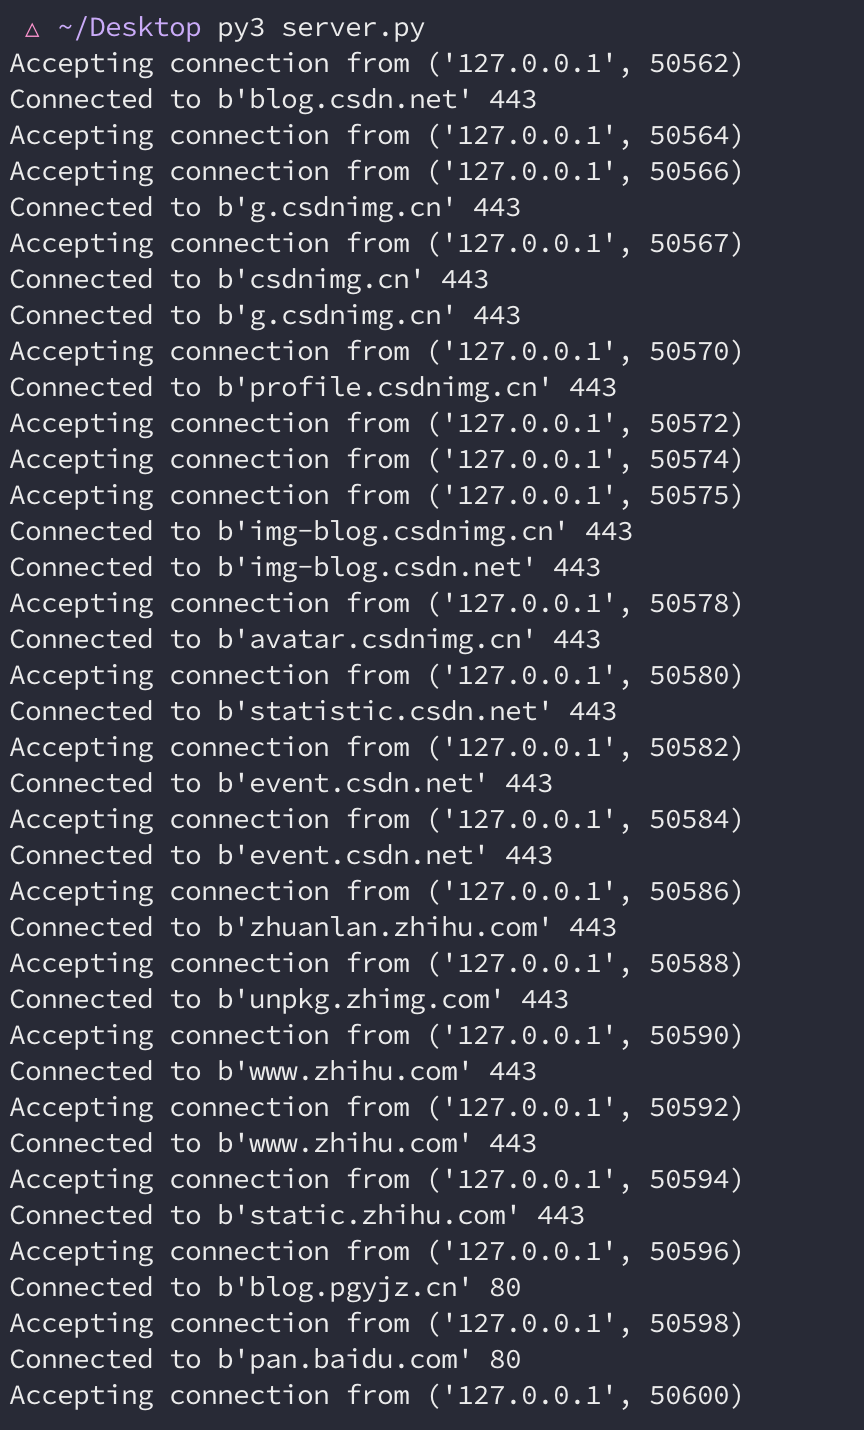
\includegraphics[scale=0.5]{ot1.png}\\
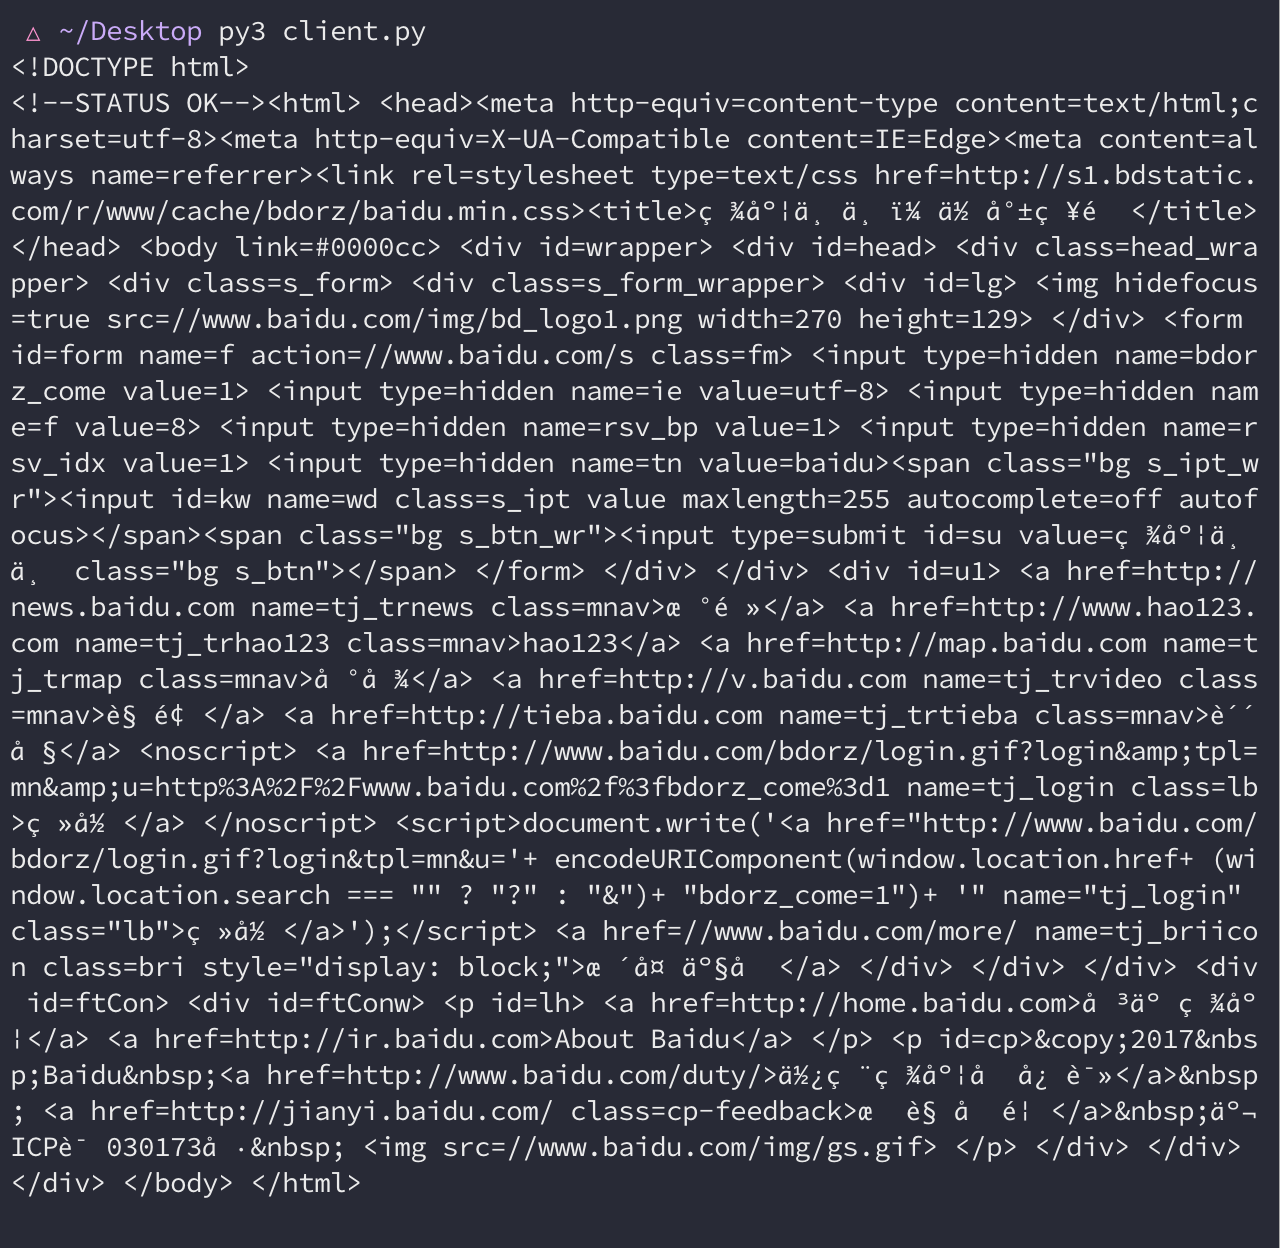
\includegraphics[scale=0.5]{ot2.png}\\
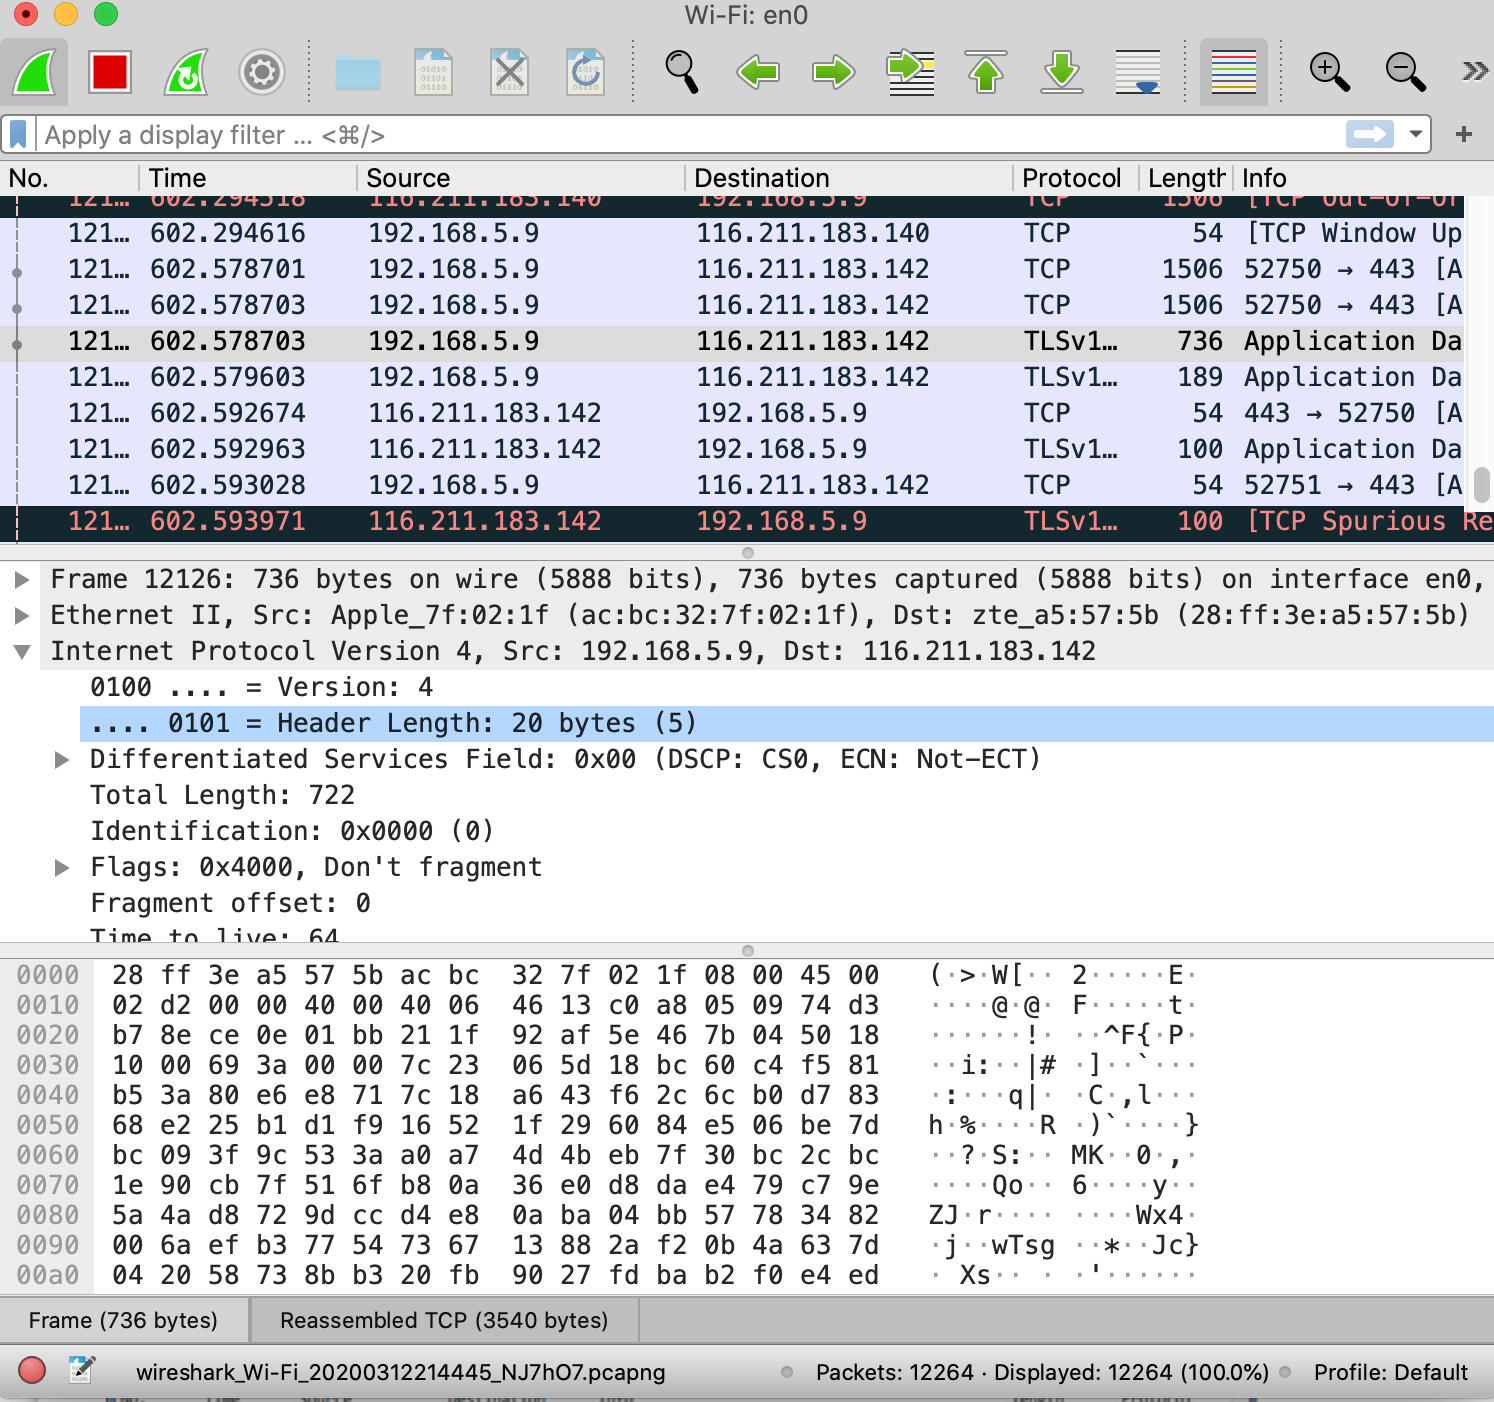
\includegraphics[scale=0.5]{ot3.png}
\end{document}
